\documentclass[12pt,twoside]{book}

\usepackage[utf8]{inputenc}
\usepackage[turkish]{babel}
\usepackage[T1]{fontenc}

\usepackage{amsmath}
\usepackage{amssymb}
\usepackage{amsthm}
\usepackage{enumerate}
\usepackage[most]{tcolorbox}

\usepackage{circuitikz}
\usepackage{cancel}
\usepackage{bodegraph}
\usepackage{gensymb}

\usepackage{verbatim}
\usepackage{listings}
\usepackage{matlab-prettifier}

\usepackage{pgfplots}
\pgfplotsset{compat=newest}
\usepackage{pgffor}
\usepackage{xcolor}

\usepackage{tikz}
\usetikzlibrary{patterns}
\usetikzlibrary{babel}

\usetikzlibrary{shapes.misc}
\tikzset{cross/.style={cross out, draw=black, minimum size=2*(#1-\pgflinewidth), inner sep=0pt, outer sep=0pt},
%default radius will be 3pt. 
cross/.default={3pt}}
\usetikzlibrary{arrows}
\tikzset{
  arrow/.pic={\path[tips,every arrow/.try,->,>=#1] (0,0) -- +(.1pt,0);},
  pics/arrow/.default={triangle 90}
}

\usepackage{siunitx}
\usepackage{textcomp}

\usepackage{hyperref}
\hypersetup{
    colorlinks=true,
    linkcolor=blue,
    filecolor=magenta,      
    urlcolor=cyan,
    pdftitle={Kitap},
    pdfpagemode=FullScreen,
    }

\urlstyle{same}

\usepackage{graphicx}
\graphicspath{{svg-inkscape/}}
\usepackage{geometry}
\usepackage{subcaption}
\usepackage{tabularray}
\usepackage{tabularx}
\DefTblrTemplate{contfoot-text}{default}{Bir sonraki sayfada devam ediyor.} % Uzun Tablolar için alt kısım
\DefTblrTemplate{conthead-text}{default}{(Devam)} % Uzun Tablolar için üst kısım

\usepackage{lscape}

\usepackage{pgfplotstable}
\usepackage{booktabs}

\usepackage{steinmetz}
\usepackage{matlab-prettifier}
\usepackage[tc]{titlepic}


\begin{document}
\shorthandoff{=} % babel paketi hatasını gidermek için gerekli
\renewcommand{\chaptername}{Bölüm}
\renewcommand{\contentsname}{İçindekiler}
\renewcommand{\figurename}{Şekil}
\renewcommand{\tablename}{Çizelge}
\renewcommand{\bibname}{Kaynaklar}
\renewcommand{\listfigurename}{Şekiller}
\renewcommand{\listtablename}{Çizelgeler}
\renewcommand{\appendixname}{Ek}
\renewcommand{\indexname}{Dizin}
\renewcommand{\partname}{Bölüm}
\renewcommand{\proofname}{İspat}
\definecolor{other}{RGB}{171,0,255}

%%%%%%%%%%%%%%%%%%%%%%%%%%%%%%%%%%%%%%%%%%%%%%%%%%%%%%%%%%%%%%%%%%%%%%%%%%%%%%%%%%%
\title{\bfseries{\sc\textcolor{black}{Bilgisayarlı Kontrol Sistemleri \\ Ders Notu}}}
\author{\textcolor{black}{Dr. Mehmet CANEVİ} \\[5pt]
\emph{\textcolor{black}{Bilgisayar Mühendisliği}}\\[2cm]
   \vspace{2cm}
\titlepic{
\includegraphics[width=0.2\textwidth]{logo}\\[5pt]
\textcolor{black}{Niğde Ömer Halisdemir Üniversitesi}\\[5pt]
 \textcolor{black}{Türkiye}\\
 \vfill
 \textcolor{black}{2025}}}
\date{}

\lstset{language=Python, literate={-}{-}1,morekeywords={as}}
\lstset{frame=lines}
\lstset{label={lst:code_direct}}
\lstset{basicstyle=\footnotesize}
\lstset{keepspaces=true}
\lstset{columns=fullflexible}
\lstset{keywordstyle=\color{blue}}
\lstset{commentstyle=\color{green}}
\lstset{stringstyle=\color{red}}
\lstset{showspaces=false}           
\lstset{showstringspaces=false}   

\maketitle
%%%%%%%%%%%%%%%%%%%%%%%%%%%%%%%%%%%%%%%%%%%%%%%%%%%%%%%%%%%%%%%%%%%%%%%%%%%%%%%%%%%
\let \savenumberline \numberline
\def \numberline#1{\savenumberline{#1.}}
\tableofcontents

\documentclass[17pt]{beamer}

\usepackage[utf8]{inputenc}
\usepackage[turkish]{babel}
\usepackage[T1]{fontenc}

\usepackage{amsmath}
\usepackage{amssymb}
\usepackage{amsthm}
\usepackage{enumerate}
\usepackage{tikz}
\usepackage{transparent}
\usepackage{xcolor}

\usetheme{Warsaw}
\usecolortheme{default}
\definecolor{nigdeyesili_acik}{RGB}{3, 150, 166}
\definecolor{nigdeyesili_koyu}{RGB}{143, 209, 217}
\setbeamercolor{structure}{fg=nigdeyesili_acik}

\author[Dr. Mehmet CANEVİ]{Arş.~Gör.~Dr.~M.~Canevi\inst{1}}

\institute{
    \inst{1}%
    Bilgisayar Mühendisliği\\
    Mühendislik Fakültesi
}
    
\date[2025] {Ders Notları, Ocak 2025}
    
\logo{\transparent{0.4}
\includegraphics[width = 20mm]{logo}}
    
\title[Ders 1] {Kod yazma, Kod derleme. Değişken tanımlama, veri tipleri. Operatörler.}
\begin{document}
%%%%%%%%%%%%%%%%%%%%%%%%%%%%%%%%%%%%%%%%%%%%%%%%%%%%%%%%%%%%%%%%%%%%%%%%%%%%%%%%
\frame{\titlepage}
\begin{frame}[fragile]{İçidekiler}
    \tableofcontents
\end{frame}
%%%%%%%%%%%%%%%%%%%%%%%%%%%%%%%%%%%%%%%%%%%%%%%%%%%%%%%%%%%%%%%%%%%%%%%%%%%%%%%%
\section{Örnek}
\begin{frame}[fragile]
    \lstinputlisting{lec1/main.c}
\end{frame}
%%%%%%%%%%%%%%%%%%%%%%%%%%%%%%%%%%%%%%%%%%%%%%%%%%%%%%%%%%%%%%%%%%%%%%%%%%%%%%%%
\section{Kod yazma}
\begin{frame}[fragile]{Kod nedir?}
    Bilgisayar tanımı kapsamına giren cihazlara meramımızı anlatmak için yazılan şeye \textbf{kod} diyebiliriz.
\end{frame}
%%%%%%%%%%%%%%%%%%%%%%%%%%%%%%%%%%%%%%%%%%%%%%%%%%%%%%%%%%%%%%%%%%%%%%%%%%%%%%%%
\section{Değişken tanımlama ve veri tipleri}
\begin{frame}[fragile]{Değişken isimleri}
    Değişkenler şu şekilde tanımlanmaktadır:
    \begin{lstlisting}
        veri_tipi degisken_adi;
        veri_tipi degisken_adi=ilk_deger;\end{lstlisting}
    Buradaki \lstinline{veri_tipi};
    \begin{itemize}
        \item \lstinline{int} 
        \item \lstinline{float}
        \item \lstinline{double}
        \item \lstinline{char}
    \end{itemize}
     olabilmektedir. \lstinline{degisken_adi} ise 
    \begin{itemize}
     \item türkçe karakter içermemelidir
     \item sadece harf veya alttire ile başlamalıdır
     \item özel karakterler(!,?,vb.) ve boşluk içermemelidir
     \item \lstinline{veri_tipi} anahtar kelimeleri olmamalıdır
    \end{itemize}
    kurallarına uymalıdır.
\end{frame}
%%%%%%%%%%%%%%%%%%%%%%%%%%%%%%%%%%%%%%%%%%%%%%%%%%%%%%%%%%%%%%%%%%%%%%%%%%%%%%%%
\begin{frame}[fragile]{Değişken tiplerinin anlamı}
    Değişkenler
    \begin{itemize}
     \item \lstinline{int} ingilizce \verb|integer| yani tam sayıdan gelmektedir \lstinline{-10,4} gibi
     \item \lstinline{float} ingilizcede kayan noktalı sayı(6-7 basamak) anlamındadır \lstinline{3.14f} gibi
     \item \lstinline{double} ingilizcede iki kat hassasiyet(15 basamak) anlamındadır \lstinline{3.14} gibi
     \item \lstinline{char} ingilizce \verb|character|'den gelir \lstinline{'c','x'} gibi
    \end{itemize}
    veri tipleri ile tanımlanabilmektedir ve 
    \begin{itemize}
        \item \lstinline{int var1=-10;} 
        \item \lstinline{float var2=3.14f;} 
        \item \lstinline{double var3=3.14;} 
        \item \lstinline{char var4='x';} 
    \end{itemize}
    olarak örneklendirilebilir.
\end{frame}
%%%%%%%%%%%%%%%%%%%%%%%%%%%%%%%%%%%%%%%%%%%%%%%%%%%%%%%%%%%%%%%%%%%%%%%%%%%%%%%%
\begin{frame}[fragile]{Çoklu değişken tanımlama}
    Birden fazla değişken
    \begin{itemize}
        \item \lstinline{int a,b,c=-10;} 
        \item \lstinline{float a=2.2,b,c=3.14f;} 
        \item \lstinline{double a,b,c=3.14;} 
        \item \lstinline{char a,b,c;a=b=c='x';}
    \end{itemize}
    şeklinde tanımlanabilir.
\end{frame}
%%%%%%%%%%%%%%%%%%%%%%%%%%%%%%%%%%%%%%%%%%%%%%%%%%%%%%%%%%%%%%%%%%%%%%%%%%%%%%%%
\begin{frame}[fragile]{Değişkenlerin yazdırılması}
    Değişkenler
    \begin{itemize}
        \item \lstinline{int var1=-10;printf("%d",var1);} 
        \item \lstinline{float var2=3.14f;printf("%f",var2);} 
        \item \lstinline{double var3=3.14;printf("%lf",var3);} 
        \item \lstinline{char var4='x';printf("%c",var4);}
        \item \lstinline{printf("%s","Bu bir cumledir.");}
    \end{itemize}
    ile ekrana yazdırılır.
\end{frame}
%%%%%%%%%%%%%%%%%%%%%%%%%%%%%%%%%%%%%%%%%%%%%%%%%%%%%%%%%%%%%%%%%%%%%%%%%%%%%%%%
\begin{frame}[fragile]{Sabit değerli değişkenler}
    Değeri değişmemesi gereken değişkenler
    \begin{itemize}
        \item \lstinline{const int SAAT_DK=60;} 
        \item \lstinline{const float PI_SAYISI=3.14;} 
    \end{itemize}
    şeklinde tanımlanır ve büyük harflerin kullanımı bir gelenektir. Dolayısıyla,
    \begin{itemize}
        \item \lstinline{SAAT_DK=120;} 
        \item \lstinline{PI_SAYISI=5.5;} 
    \end{itemize}
    hata verir.
\end{frame}
%%%%%%%%%%%%%%%%%%%%%%%%%%%%%%%%%%%%%%%%%%%%%%%%%%%%%%%%%%%%%%%%%%%%%%%%%%%%%%%%
\section{Operatörler}
\begin{frame}[fragile]{Matematiksel operatörler}
    Toplama ve çıkarma işlemi
    \begin{itemize}
        \item \lstinline{int a=4+5;int c=a-2;int d=a+c;} 
    \end{itemize}
    ile örneklendirilebilir. Matematiksel operatörler
    \begin{itemize}
        \item \lstinline{+,-} toplama, çıkarma 
        \item \lstinline{*,/} çarpma, bölme
        \item \lstinline{++,--} arttırma, azaltma 
        \item \lstinline{%} \verb|mod| operatörü (bölümden kalan)
        \item \lstinline{=} atama operatörü
    \end{itemize}
    şeklindedir.
\end{frame}
%%%%%%%%%%%%%%%%%%%%%%%%%%%%%%%%%%%%%%%%%%%%%%%%%%%%%%%%%%%%%%%%%%%%%%%%%%%%%%%%
\begin{frame}[fragile]{Matematiksel operatörler(devam)}
    Aşağıdaki operatörler tanımlıdır.
    \begin{itemize}
        \item \lstinline{x+=3;} \lstinline{x=x+3;} 
        \item \lstinline{x-=3;} \lstinline{x=x-3;} 
        \item \lstinline{x*=3;} \lstinline{x=x*3;} 
        \item \lstinline{x/=3;} \lstinline{x=x/3;} 
        \item \lstinline{x%=3;} \lstinline{x=x%3;} 
    \end{itemize}
\end{frame}
%%%%%%%%%%%%%%%%%%%%%%%%%%%%%%%%%%%%%%%%%%%%%%%%%%%%%%%%%%%%%%%%%%%%%%%%%%%%%%%%
\begin{frame}[fragile]{Karşılaştırma operatörleri}
    Aşağıdaki operatörler ile karşılaştırma başarılı ise 1 değilse sıfır değerini alır.
    \begin{itemize}
        \item \lstinline{x>y} Büyüktür
        \item \lstinline{x>=y} Büyük eşittir
        \item \lstinline{x<y} Küçüktür
        \item \lstinline{x<=y} Küçük eşittir
        \item \lstinline{x==y} Eşittir
        \item \lstinline{x!=y} Eşit değildir
    \end{itemize}
\end{frame}
%%%%%%%%%%%%%%%%%%%%%%%%%%%%%%%%%%%%%%%%%%%%%%%%%%%%%%%%%%%%%%%%%%%%%%%%%%%%%%%%
\begin{frame}[fragile]{Mantıksal operatörleri}
    Mantıksal operatörler
    \begin{itemize}
        \item \lstinline{sart1 && sart2} VE
        \item \lstinline{sart1 || sart2} VEYA 
        \item \lstinline{!sart} DEĞİLDİR 
    \end{itemize}
    olarak verilmiştir.
\end{frame}
%%%%%%%%%%%%%%%%%%%%%%%%%%%%%%%%%%%%%%%%%%%%%%%%%%%%%%%%%%%%%%%%%%%%%%%%%%%%%%%%
\end{document}
\chapter{Ayrıklaştırma}
Türevin geometrik yorumu 
\begin{equation}
    \frac{dy(t)}{dt}\approx\frac{\Delta y}{\Delta t}
\end{equation}
olmak üzere
\begin{equation}
\begin{split}
    \frac{dy(t)}{dt}&\approx\frac{\Delta y}{\Delta t}\\
    &\approx\frac{y((k+1)T)-y(kT)}{(k+1)T-kT}\\
    &\approx\frac{y((k+1)T)-y(kT)}{T}
\end{split}
\end{equation}
elde edilir. Ayrık bir sinyalin türevi ardışık değerler farkının örnekleme zamanına oranı ile hesaplanabilmektedir. Örneğin, $y(kT)=\sin(kT)$ ve $T=0.1$ olmak üzere
\begin{equation}
    \frac{y((k+1)T)-y(kT)}{T}=10(\sin((k+1)0.1)-\sin(0.1k))
\end{equation}
ve dolayısıyla
\begin{equation}
\begin{split}
    \{10\sin(0.1),10(\sin(0.2)-\sin(0.1)),10(\sin(0.3)-\sin(0.2)),\cdots\}\\
    \{0.9983,0.9884, 0.9685,\cdots\}
\end{split}
\end{equation}
elde edilir. $y(kT)=\sin(kT)$ sinyalinin türevinin $\frac{d\sin(t)}{dt}=\cos(t)$ olduğu bilindiğinden
\begin{equation}
    \begin{split}
        \{cos(0.1),cos(0.2),cos(0.3),\cdots\}\\
        \{ 0.9950,0.9801,0.9553,\cdots\}
    \end{split}
\end{equation}
elde edilir ve ayrık türev ile benzer değerler olduğu görülmektedir. Bu yaklaşıklığın türeve yakınsaması için örnekleme zamanı $T$ daha küçük seçilmelidir. 
\begin{equation}
    \frac{dq(t)}{dt}=x
\end{equation}
olmak üzere
\begin{equation}
\begin{split}
    \frac{dq(t)}{dt}&=x\\
    dq(t)&=xdt\\
    \int dq(t)&=\int xdt\\
    q(t)&=\int xdt
\end{split}
\end{equation}
elde edilir. Buradan hareketle,
\begin{equation}
    \begin{split}
        \frac{\Delta q}{\Delta t}&=x\\
        \frac{q((k+1)T)-q(kT)}{(k+1)T-kT}&=x\\
        \frac{q((k+1)T)-q(kT)}{T}&=x\\
        q((k+1)T)-q(kT)&=xT\\
        q((k+1)T)&=q(kT)+xT
    \end{split}
\end{equation}
ifadesi bulunur. Ayrık zamanda integral birikimli toplama karşılık gelmektedir. Bu karşılıklar Zero Order Hold(ZOH) ile elde edilmiştir. ZOH örnekleme zamanı boyunca değerlerin sabit olduğu varsayımına dayanmaktadır. Bu durum
\begin{equation}
    x(t)=x(kT),\quad kT\leq t\leq (k+1)T
\end{equation}
ile ifade edilebilir.

First Order Hold(FOH) yöntemi ise
\begin{equation}
    x(t)=x(kT)+\frac{t-kT}{T}(x((k+1)T)-x(kT)),\quad kT\leq t\leq (k+1)T
\end{equation}
olarak tanımlanır. Eşitliğin sağ tarafı $t=kT$ için $x(kT)$, $t=(k+0.5)T$ için 
\begin{equation}
\begin{split}
    x(t)&=x(kT)+\frac{t-kT}{T}(x((k+1)T)-x(kT)),\quad kT\leq t\leq (k+1)T\\
    &=x(kT)+\frac{kT+0.5T-kT}{T}(x((k+1)T)-x(kT))\\
    &=x(kT)+0.5(x((k+1)T)-x(kT))\\
    &=x(kT)+0.5x((k+1)T)-0.5x(kT)\\
    &=0.5x((k+1)T)+0.5x(kT)
\end{split}
\end{equation}
ve $t=(k+1)T$ için ise 
\begin{equation}
    \begin{split}
        x(t)&=x(kT)+\frac{t-kT}{T}(x((k+1)T)-x(kT)),\quad kT\leq t\leq (k+1)T\\
        x(t)&=x(kT)+\frac{(k+1)T-kT}{T}(x((k+1)T)-x(kT))\\
        x(t)&=x(kT)+x((k+1)T)-x(kT)\\
        x(t)&=x((k+1)T)
    \end{split}
\end{equation}
elde edilir. Görüldüğü üzere ZOH yönteminin aksine $T$ süre boyunca değerler değişmektedir.
\chapter{Fark Denklemleri}
Örnek sistemin ZOH yöntemi ile elde edilen ve Denklem~\ref{eqn:ornek_sistem_zoh} ile verilen sistem için
\begin{equation}
\begin{split}
    G_{ZOH}(z)&=\frac{1-e^{-1}}{z-e^{-1}}\\
    &=\frac{(1-e^{-1})z^{-1}}{1-e^{-1}z^{-1}}\\
    \frac{y(z)}{u(z)}&=\frac{(1-e^{-1})z^{-1}}{1-e^{-1}z^{-1}}\\
    y(z)(1-e^{-1}z^{-1})&=(1-e^{-1})z^{-1}u(z)\\
    y(z)-y(z-1)e^{-1}&=(1-e^{-1})u(z-1)\\
    y(z)&=y(z-1)e^{-1}+(1-e^{-1})u(z-1)\\
    y(z)&=0.3679y(z-1)+0.6321u(z-1)
\end{split}
\end{equation}
elde edilir. Z tanım bölgesinde tanımlı transfer fonksiyonundan fark denklemine geçişe örnektir. Fark denklemleri programlama dilleri ile kolaylıkla gerçeklenebilmektedir.
Benzer şekilde FOH yöntemi ile elde edilen ve Denklem~\ref{eqn:ornek_sistem_foh} ile verilen ifade için
\begin{equation}
    \begin{split}
        G_{FOH}(z)&=\frac{1}{z}\\
        \frac{y(z)}{u(z)}&=z^{-1}\\
        y(z)&=u(z-1)
    \end{split}
\end{equation}
elde edilir.
Yay-Kütle-Damper sistemi için dinamikleri ifade eden denklem
\begin{equation}
    m\ddot{x}(t)+b\dot{x}(t)+kx(t)=u(t)\label{eqn:mass_spring_damper}
\end{equation}
olarak verilmiştir. Bu diferansiyel denklem S tanım bölgesine dönüştürülürse
\begin{equation}
\begin{split}
    ms^2X(s)+b sX(s)+kX(s)&=U(s)\\
    (ms^2+b s+k)X(s)&=U(s)\\
    \frac{X(s)}{U(s)}=\frac{1}{ms^2+b s+k}
\end{split}
\end{equation}
elde edilir. Denklem~\ref{eqn:mass_spring_damper} ile verilen sistem için 
\begin{gather}
    m\frac{\Delta^2 x}{(\Delta t)^2}+b\frac{\Delta x}{\Delta t}+kx(kT)=u(kT)\nonumber\\
    m\frac{\Delta (x(kT)-x((k-1)T))}{kT-(k-1)T}+b\frac{x(kT)-x((k-1)T)}{kT-(k-1)T}+kx(kT)=u(kT)\nonumber\\
    m\frac{\Delta x(kT)-\Delta x((k-1)T)}{T^2}+b\frac{x(kT)-x((k-1)T)}{T}+kx(kT)=u(kT)\nonumber\\
    m\frac{x(kT)-2x((k-1)T)+x((k-2)T)}{T^2}+b\frac{x(kT)-x((k-1)T)}{T}+kx(kT)=u(kT)\nonumber\\
    m\frac{x(kT)-2x((k-1)T)+x((k-2)T)}{T^2}+b\frac{x(kT)-x((k-1)T)}{T}+kx(kT)=u(kT)\nonumber\\
    (m+bT+kT^2)x(kT)=(2m+bT)x((k-1)T)-mx((k-2)T)+T^2u(kT)\nonumber\\
    x(kT)=\frac{2m+bT}{m+bT+kT^2}x((k-1)T)-\frac{m}{m+bT+kT^2}x((k-2)T)+\frac{T^2}{m+bT+kT^2}u(kT)
\end{gather}
Örnek olması için $m=1\,kg$, $b=1\,Ns/m$, $k=1\,Nm$ ve $T=0.1$ olmak üzere fark denklemi
\begin{equation}
    x(kT)=1.8919x((k-1)T)-0.9009x((k-2)T)+0.009009u(kT)
\end{equation}
olarak elde edilir. Transfer fonksiyonundan yola çıkarak $\zeta=b\sqrt{m}/(2m\sqrt{k})$, $w_n=\sqrt{k}/\sqrt{m}$ ve $\phi=\cos^{-1}(\zeta)$ olmak üzere
\begin{equation}
\begin{split}
    G(z)&=\mathcal{Z}\left\{\frac{1-e^{-0.1s}}{s(s^2+s+1)}\right\}\\
    &=\frac{z-1}{z}\mathcal{Z}\left\{\frac{1}{s(s^2+s+1)}\right\}\\
    &=\frac{z-1}{z}\left(\frac{z}{z-1}-\frac{1}{\sqrt{1-\zeta^2}}\frac{\sqrt{1-\zeta^2}z^2+ze^{-\zeta w_nT}\sin(w_n\sqrt{1-\zeta^2}T-\phi)}{z^2-2ze^{-\zeta w_nT}\cos(w_n\sqrt{1-\zeta^2}T)+e^{-2\zeta w_nT}}\right)\\
    &=\frac{0.004833 z^3 - 0.0001585 z^2 - 0.004675 z}{ z^4 - 2.895 z^3 + 2.8 z^2 - 0.9048 z}\\
    &=\frac{0.004833 z + 0.004675}{z^2 - 1.895 z + 0.9048}
\end{split}
\end{equation}
elde edilir.
\begin{enumerate}
    \item Yay-kütle-damper sisteminin çıkış işaretini fark denklemlerini kullanarak elde ediniz. 
    \begin{lstlisting}
    m=1
    b=1
    k=1
    T=0.1
    fac1=(2*m+b*T)/(m+b*T+k*T**2)
    fac2=-m/(m+b*T+k*T**2)
    fac3=T**2/(m+b*T+k*T**2)
    tvec=np.arange(0,10+1,T)
    xt=np.zeros(tvec.shape)
    ut=np.ones(tvec.shape)
    for i in range(0,len(tvec)):
        if i==0:
            xt[i]=fac1*0+fac2*0+fac3*0
        elif i==1:
            xt[i]=fac1*xt[i-1]+fac2*0+fac3*ut[i-1]
        else:
            xt[i]=fac1*xt[i-1]+fac2*xt[i-2]+fac3*ut[i-1]

    plt.grid('minor')
    plt.xlabel("Zaman(s)")
    plt.ylabel("x(t)")
    plt.title("Yay-kutle-damper sistem yaniti")

    Gz=control.tf(1,np.array([m,b,k]))
    tc, yc=control.step_response(Gz)
    plt.plot(tc,yc,'k')
    plt.stem(tvec,xt,'b')
    plt.show()
    \end{lstlisting}

    \begin{figure}[!htb]
        \centering
        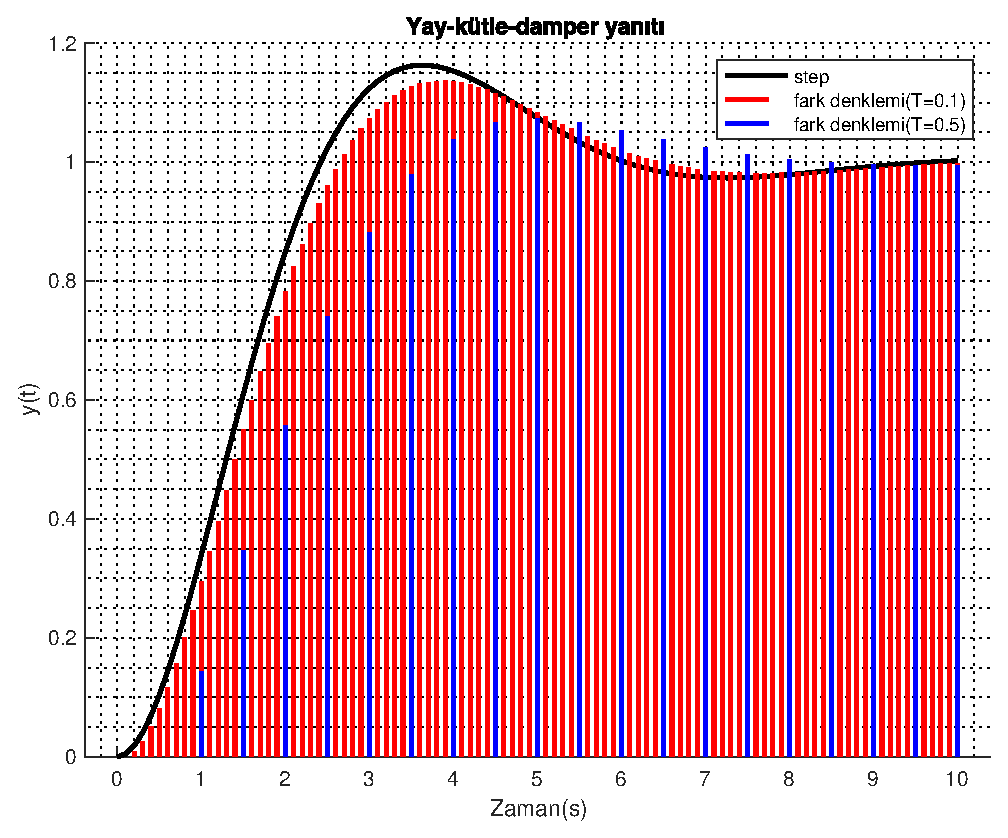
\includegraphics[width=0.5\textwidth]{img/lec3_step1}
        \caption{Yay-kütle-damper sisteminin çıkış işareti}
        \label{fig:lec3_step1}
    \end{figure}
    \item Yay-kütle-damper sisteminin çıkış işaretini ayrık transfer fonksiyonu kullanarak elde ediniz. 
    \begin{lstlisting}
    m=1
    b=1
    k=1
    
    plt.grid('minor')
    plt.xlabel("Zaman(s)")
    plt.ylabel("x(t)")
    plt.title("Yay-kutle-damper sistem yaniti")

    Gz=control.tf(1,np.array([m,b,k]))
    tc, yc=control.step_response(Gz)

    Gz1=control.c2d(control.tf(1,np.array([m,b,k])),0.1)
    tc1, yc1=control.step_response(Gz1)

    Gz2=control.c2d(control.tf(1,np.array([m,b,k])),0.5)
    tc2, yc2=control.step_response(Gz2)

    plt.plot(tc,yc,'k')
    plt.stem(tc1,yc1,'r')
    plt.stem(tc2,yc2,'b')
    plt.show()
    \end{lstlisting}
    \begin{figure}[!htb]
        \centering
        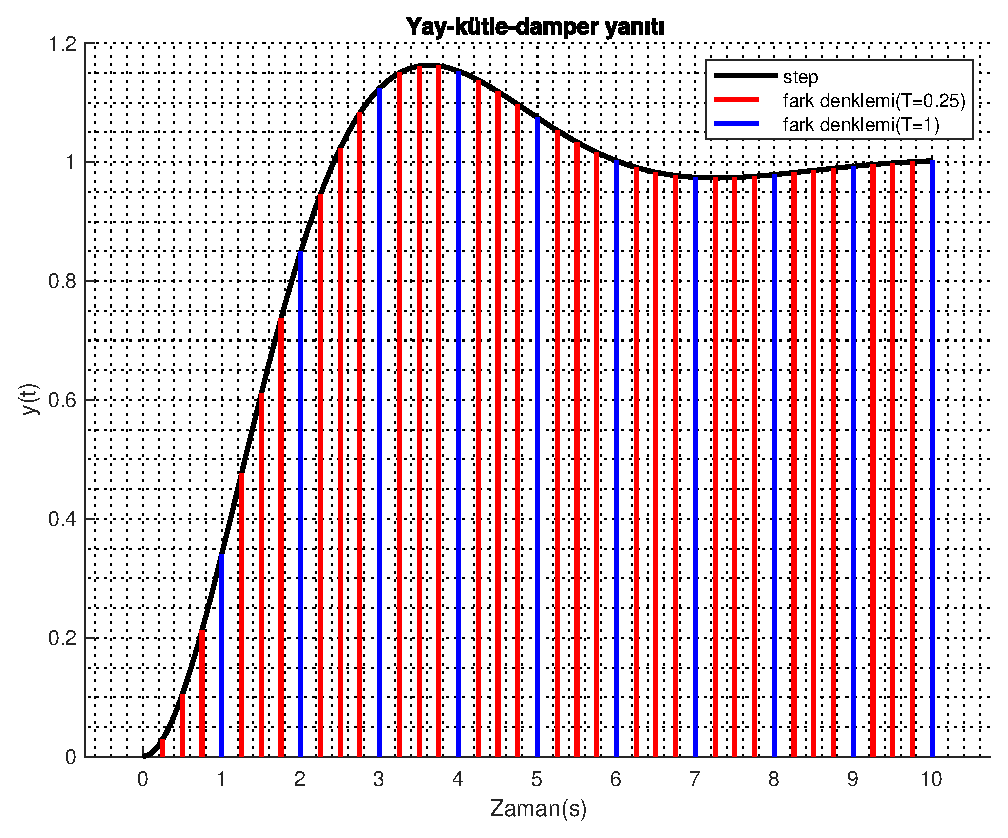
\includegraphics[width=0.5\textwidth]{img/lec3_step2}
        \caption{Yay-kütle-damper sisteminin çıkış işareti}
        \label{fig:lec3_step2}
    \end{figure}
\end{enumerate}
\documentclass[17pt]{beamer}

\usepackage[utf8]{inputenc}
\usepackage[turkish]{babel}
\usepackage[T1]{fontenc}

\usepackage{amsmath}
\usepackage{amssymb}
\usepackage{amsthm}
\usepackage{enumerate}
\usepackage{tikz}
\usepackage{transparent}
\usepackage{xcolor}

\usetheme{Warsaw}
\usecolortheme{default}
\definecolor{nigdeyesili_acik}{RGB}{3, 150, 166}
\definecolor{nigdeyesili_koyu}{RGB}{143, 209, 217}
\setbeamercolor{structure}{fg=nigdeyesili_acik}

\author[Dr. Mehmet CANEVİ]{Arş.~Gör.~Dr.~M.~Canevi\inst{1}}

\institute{
    \inst{1}%
    Bilgisayar Mühendisliği\\
    Mühendislik Fakültesi
}
    
\date[2025] {Ders Notları, Ocak 2025}
    
\logo{\transparent{0.4}
\includegraphics[width = 20mm]{logo}}
    
\title[Ders 4] {Diziler I}
\begin{document}
%%%%%%%%%%%%%%%%%%%%%%%%%%%%%%%%%%%%%%%%%%%%%%%%%%%%%%%%%%%%%%%%%%%%%%%%%%%%%%%%
\frame{\titlepage}
\begin{frame}[fragile]{İçidekiler}
    \tableofcontents
\end{frame}
%%%%%%%%%%%%%%%%%%%%%%%%%%%%%%%%%%%%%%%%%%%%%%%%%%%%%%%%%%%%%%%%%%%%%%%%%%%%%%%%
\section{Dizileri tanıyalım}
\begin{frame}[fragile]{Fibbonacci sayıları}
    Fibbonacci sayılarını tanımlayalım: 
    \begin{lstlisting}
        int fibb1=1;    
        int fibb2=1;    
        int fibb3=2;    
        int fibb4=3;    
        int fibb5=5;    
        int fibb6=8;    
        int fibb7=13;\end{lstlisting}
    Dizinin 100 terimi için 100 adet değişken gerekirdi. Bu noktada diziler kullanılır.
\end{frame}
%%%%%%%%%%%%%%%%%%%%%%%%%%%%%%%%%%%%%%%%%%%%%%%%%%%%%%%%%%%%%%%%%%%%%%%%%%%%%%%%
\begin{frame}[fragile]{Diziler}
    Diziler kullanılırsa
    \begin{lstlisting}
        int fibb[]={1,1,2,3,5,8,13};\end{lstlisting}
        ile tanımlanır. Tanımlama şekli
    \begin{lstlisting}
        veri_tipi degisken_adi[]={x1,x2,x3,x4,...};
        veri_tipi degisken_adi[3]={x1,x2,x3};
        veri_tipi degisken_adi[dizi_uzunlugu];
    \end{lstlisting}
    olarak verilebilir.
\end{frame}
%%%%%%%%%%%%%%%%%%%%%%%%%%%%%%%%%%%%%%%%%%%%%%%%%%%%%%%%%%%%%%%%%%%%%%%%%%%%%%%%
\begin{frame}[fragile]{Fibbonacci Dizileri(devam)}
    Fibbonacci dizisi 
    \begin{lstlisting}
        int fibb[5];
        int i;
        fibb[0]=1;
        fibb[1]=1;
        for(i=2;i<5;i++)
        {
            fibb[i]=fibb[i-1]+fibb[i-2];
        }
    \end{lstlisting}
\end{frame}
%%%%%%%%%%%%%%%%%%%%%%%%%%%%%%%%%%%%%%%%%%%%%%%%%%%%%%%%%%%%%%%%%%%%%%%%%%%%%%%%
\begin{frame}[fragile]{Fibbonacci Dizileri(devam)}
    Fibbonacci dizisi 
    \begin{lstlisting}
        fibb[0]=1;
        fibb[1]=1;
        fibb[2]=fibb[1]+fibb[0];
        fibb[3]=fibb[2]+fibb[1];
        fibb[4]=fibb[3]+fibb[2];
    \end{lstlisting}
\end{frame}
%%%%%%%%%%%%%%%%%%%%%%%%%%%%%%%%%%%%%%%%%%%%%%%%%%%%%%%%%%%%%%%%%%%%%%%%%%%%%%%%
\begin{frame}[fragile]{2 boyutlu diziler}
    2 boyutlu diziler
    \begin{lstlisting}
        veri_tipi degisken_adi[][]={{x11,x12,x13,...},{x21,x22,x23,...},...};
        veri_tipi degisken_adi[3][3]={{1,0,0},{0,1,0},{0,0,1}};
        veri_tipi degisken_adi[dizi_uzunlugu][dizi_uzunlugu];
    \end{lstlisting}
    ile tanımlanır.
\end{frame}
%%%%%%%%%%%%%%%%%%%%%%%%%%%%%%%%%%%%%%%%%%%%%%%%%%%%%%%%%%%%%%%%%%%%%%%%%%%%%%%%
\begin{frame}[fragile]{n boyutlu diziler}
    n boyutlu diziler
    \begin{lstlisting}
        veri_tipi degisken_adi[x][y][z]...={{{},{},...},{{},{},...},....};
        veri_tipi degisken_adi[x][y][z]...;
    \end{lstlisting}
    ile tanımlanır.
\end{frame}

%%%%%%%%%%%%%%%%%%%%%%%%%%%%%%%%%%%%%%%%%%%%%%%%%%%%%%%%%%%%%%%%%%%%%%%%%%%%%%%%
\section{Alıştırmalar}
\begin{frame}[fragile]{Sorular}
    \begin{alertblock}{Soru-1}
        Soru
    \end{alertblock}
\end{frame}
%%%%%%%%%%%%%%%%%%%%%%%%%%%%%%%%%%%%%%%%%%%%%%%%%%%%%%%%%%%%%%%%%%%%%%%%%%%%%%%%
\end{document}
\documentclass[17pt]{beamer}

\usepackage[utf8]{inputenc}
\usepackage[turkish]{babel}
\usepackage[T1]{fontenc}

\usepackage{amsmath}
\usepackage{amssymb}
\usepackage{amsthm}
\usepackage{enumerate}
\usepackage{tikz}
\usepackage{transparent}
\usepackage{xcolor}

\usetheme{Warsaw}
\usecolortheme{default}
\definecolor{nigdeyesili_acik}{RGB}{3, 150, 166}
\definecolor{nigdeyesili_koyu}{RGB}{143, 209, 217}
\setbeamercolor{structure}{fg=nigdeyesili_acik}

\author[Dr. Mehmet CANEVİ]{Arş.~Gör.~Dr.~M.~Canevi\inst{1}}

\institute{
    \inst{1}%
    Bilgisayar Mühendisliği\\
    Mühendislik Fakültesi
}
    
\date[2025] {Ders Notları, Ocak 2025}
    
\logo{\transparent{0.4}
\includegraphics[width = 20mm]{logo}}
    
\title[Ders 5] {Diziler II}
\begin{document}
%%%%%%%%%%%%%%%%%%%%%%%%%%%%%%%%%%%%%%%%%%%%%%%%%%%%%%%%%%%%%%%%%%%%%%%%%%%%%%%%
\frame{\titlepage}
\begin{frame}[fragile]{İçidekiler}
    \tableofcontents
\end{frame}
%%%%%%%%%%%%%%%%%%%%%%%%%%%%%%%%%%%%%%%%%%%%%%%%%%%%%%%%%%%%%%%%%%%%%%%%%%%%%%%%
\section{Diziler yeniden}

\begin{frame}[fragile]{Dizi tanımlama}
    \begin{lstlisting}
        int len=8176*1024-10*1024;
        printf("len:%d\n",len);
        char dizi[len];
        int i=0;
        for(i=0;i<len;i++)
        {
            dizi[i]='x';
        }\end{lstlisting}
    ve
    \begin{lstlisting}
        int len=8176*1024;
        printf("len:%d\n",len);
        char dizi[len];
        int i=0;
        for(i=0;i<len;i++)
        {
            dizi[i]='x';
        }\end{lstlisting}
\end{frame}
%%%%%%%%%%%%%%%%%%%%%%%%%%%%%%%%%%%%%%%%%%%%%%%%%%%%%%%%%%%%%%%%%%%%%%%%%%%%%%%%
\begin{frame}[fragile]{Pointer(İşaretçi)}
    Bellek adresi için kullanılan veri tipine \textbf{pointer} denir.
    \begin{lstlisting}
    veri_tipi* degisken;    
    veri_tipi* degisken[];\end{lstlisting}
    ile tanımlanabilirler. Aynı zamanda
    \begin{lstlisting}
        veri_tipi degisken;    
        veri_tipi* adres=&degisken;\end{lstlisting}
    ile de kullanılabilir.
\end{frame}
%%%%%%%%%%%%%%%%%%%%%%%%%%%%%%%%%%%%%%%%%%%%%%%%%%%%%%%%%%%%%%%%%%%%%%%%%%%%%%%%
\end{document}
\documentclass[17pt]{beamer}

\usepackage[utf8]{inputenc}
\usepackage[turkish]{babel}
\usepackage[T1]{fontenc}

\usepackage{amsmath}
\usepackage{amssymb}
\usepackage{amsthm}
\usepackage{enumerate}
\usepackage{tikz}
\usepackage{transparent}
\usepackage{xcolor}

\usetheme{Warsaw}
\usecolortheme{default}
\definecolor{nigdeyesili_acik}{RGB}{3, 150, 166}
\definecolor{nigdeyesili_koyu}{RGB}{143, 209, 217}
\setbeamercolor{structure}{fg=nigdeyesili_acik}

\author[Dr. Mehmet CANEVİ]{Arş.~Gör.~Dr.~M.~Canevi\inst{1}}

\institute{
    \inst{1}%
    Bilgisayar Mühendisliği\\
    Mühendislik Fakültesi
}
    
\date[2025] {Ders Notları, Ocak 2025}
    
\logo{\transparent{0.4}
\includegraphics[width = 20mm]{logo}}
    
\title[Ders 6] {Struct Yapılar ve Makrolar}
\begin{document}
%%%%%%%%%%%%%%%%%%%%%%%%%%%%%%%%%%%%%%%%%%%%%%%%%%%%%%%%%%%%%%%%%%%%%%%%%%%%%%%%
\frame{\titlepage}
\begin{frame}[fragile]{İçidekiler}
    \tableofcontents
\end{frame}
%%%%%%%%%%%%%%%%%%%%%%%%%%%%%%%%%%%%%%%%%%%%%%%%%%%%%%%%%%%%%%%%%%%%%%%%%%%%%%%%
\section{Struct yapısı}
\begin{frame}[fragile]{Struct(Yapı) nedir?}
    \begin{lstlisting}
        void fonksiyon(char* isim,char* soyisim,int yas,int cinsiyet);
    \end{lstlisting}
    fonksiyonu
    \begin{lstlisting}
        struct kisi{
            char* isim;
            char* soyisim;
            int yas;
            int cinsiyet;
        };
        void fonksiyon(struct kisi k);\end{lstlisting}
    olarak da yazılabilir.
\end{frame}
%%%%%%%%%%%%%%%%%%%%%%%%%%%%%%%%%%%%%%%%%%%%%%%%%%%%%%%%%%%%%%%%%%%%%%%%%%%%%%%%
\begin{frame}[fragile]{Struct(Yapı) nedir?}
    Böylece
    \begin{lstlisting}
        struct kisi{
            char* isim;
            char* soyisim;
            int yas;
            int cinsiyet;
        };
        struct kisi fonksiyon();\end{lstlisting}
    yazılabilir.
\end{frame}
%%%%%%%%%%%%%%%%%%%%%%%%%%%%%%%%%%%%%%%%%%%%%%%%%%%%%%%%%%%%%%%%%%%%%%%%%%%%%%%%
\begin{frame}[fragile]{Struct(Yapı) nedir?}
    Basit yapı taşlarından oluşturulan karmaşık veri tipine \lstinline{struct} denir.
    \begin{lstlisting}
        struct yapi_adi{
            yapi_tasi1;
            yapi_tasi2;
            ...
        };
        struct yapi_adi degisken_adi;\end{lstlisting}
\end{frame}
%%%%%%%%%%%%%%%%%%%%%%%%%%%%%%%%%%%%%%%%%%%%%%%%%%%%%%%%%%%%%%%%%%%%%%%%%%%%%%%%
\section{Makrolar}
\begin{frame}[fragile]{define}
    Kodları kontrol etmek için kullanılır. Programın içeriğine etki etmezler.
    \begin{lstlisting}
        #define DEGISKEN\end{lstlisting}
\end{frame}
%%%%%%%%%%%%%%%%%%%%%%%%%%%%%%%%%%%%%%%%%%%%%%%%%%%%%%%%%%%%%%%%%%%%%%%%%%%%%%%%
\begin{frame}[fragile]{ifndef}
    \begin{lstlisting}
        #ifndef 1
            float a;
        #else
            double a;
        #endif\end{lstlisting}
    \lstinline{if-else} yapısının makro karşılığıdır.
\end{frame}
%%%%%%%%%%%%%%%%%%%%%%%%%%%%%%%%%%%%%%%%%%%%%%%%%%%%%%%%%%%%%%%%%%%%%%%%%%%%%%%%
\begin{frame}[fragile]{Makro fonksiyon}
    \begin{lstlisting}
        #define yazdir(str) printf(str)\end{lstlisting}
    ile fonksiyon tanımı yapılabilmektedir.
\end{frame}
%%%%%%%%%%%%%%%%%%%%%%%%%%%%%%%%%%%%%%%%%%%%%%%%%%%%%%%%%%%%%%%%%%%%%%%%%%%%%%%%
\section{Uygulama}
\begin{frame}[fragile]{Soru}
    \begin{alertblock}{Soru-1}
        Vertex struct'ı iki boyutta koordinat verisi içermektedir. Üçgen yapısı oluşturunuz. Üçgenin çevresini hesaplayan fonksiyonu yazınız.
    \end{alertblock}
    \begin{alertblock}{Soru-2}
        Matris yapısı yazınız.
    \end{alertblock}
\end{frame}
%%%%%%%%%%%%%%%%%%%%%%%%%%%%%%%%%%%%%%%%%%%%%%%%%%%%%%%%%%%%%%%%%%%%%%%%%%%%%%%%
\end{document}
\chapter{Z Tanım Bölgesinde P Kontrolör Tasarımı}
\begin{enumerate}
    \item Geçici hal yanıtını şekillendirecek isterler dikkate alınarak s tanım bölgesinde baskın kutuplar seçilir. 
    \item Baskın kutuplar $z=e^{sT}$ ilişkisi ile z tanım bölgesine aktarılır. 
    \item Kontrol edilecek sistem Z tanım bölgesine geçirilir. 
    \item Kapalı çevrim transfer fonksiyonu elde edilir ve kutup atama yapılır.
\end{enumerate}
Örnek sistem
\begin{equation}
    G(s)=\frac{1}{s+2}
\end{equation}
z tanım bölgesinde $T=0.2$ olmak üzere
\begin{equation}
    G(z)=\frac{0.1648}{z-0.6703}
\end{equation}
olarak elde edilmektedir. Yerleşme zamanı $t_s=2$ ve aşım $\%10$ isterleri verilmiştir. Bu durumda $\zeta=0.591$ ve $w_n=6.7664$ seçilir. Seçilen sönüm oranı ve doğal frekans ile baskın kutuplar
\begin{equation}
    s_{1,2}=-4 \pm 5.4575i
\end{equation}
şeklinde hesaplanır. $z=e^{sT}$ ifadesi ile z tanım bölgesinde kutuplar
\begin{equation}
    z_{1,2}=0.2072 \pm 0.3987i
\end{equation}
ve kutuplardan oluşturulacak polinom
\begin{equation}
    p(z)=z^2-0.4144 z+0.2019
\end{equation}
olarak hesaplanır. P tipi kontrolör ile kapalı çevrim transfer fonksiyonunun ifadesi
\begin{equation}
\begin{split}
    T(z)&=\frac{kG(z)}{1+kG(z)}\\
    &=\frac{k\frac{0.1648}{z-0.6703}}{1+k\frac{0.1648}{z-0.6703}}\\
    &=\frac{k(0.1648)}{z-0.6703+k(0.1648)}\\
    &=\frac{0.1648k}{z+0.1648k-0.6703}
\end{split}
\end{equation}
şeklindedir. Görüldüğü üzere karakteristik polinom birinci dereceden elde edilmiştir ve her iki isterlerin sağlanması mümkün değildir. Yerleşme zamanı sağlanmak istenirse,
\begin{equation}
    s=-\frac{4}{t_s}=-4
\end{equation}
ve z tanım bölgesinde
\begin{equation}
    z=e^{sT}=e^{-0.8}=0.4493
\end{equation}
elde edilir. Bu durumda P kontrolör
\begin{equation}
\begin{split}
    -0.1648k+0.6703&=0.4493\\
    k&=1.341
\end{split}
\end{equation}
şeklindedir. Kapalı çevrim transfer fonksiyonu
\begin{equation}
    T(z)=\frac{0.221}{z - 0.4493}
\end{equation}
şeklindedir.
\begin{figure}[!htb]
    \centering
    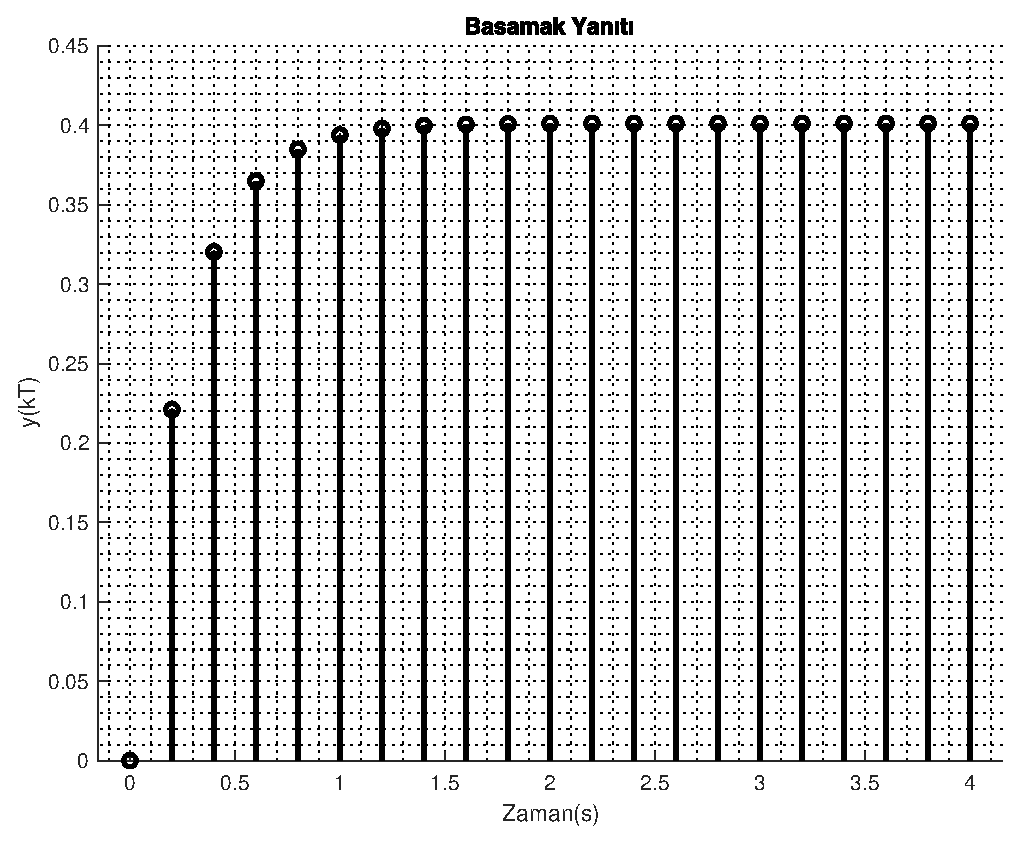
\includegraphics[width=0.75\textwidth]{img/lec7_step1}
    \caption{P kontrol için kapalı çevrim basamak yanıtı ($k=1.341$)}
    \label{fig:lec7_step1}
\end{figure}

\begin{figure}[!htb]
    \centering
    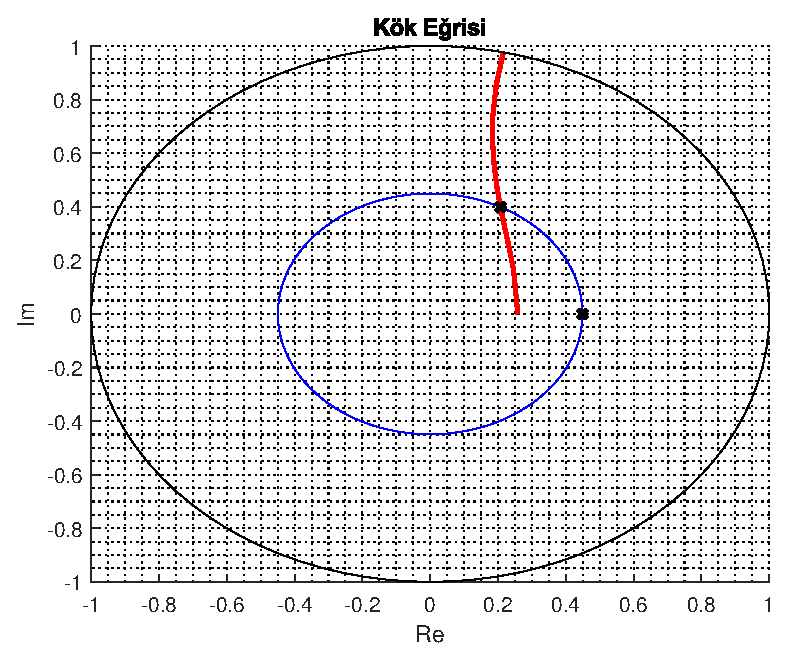
\includegraphics[width=0.75\textwidth]{img/lec7_rlocus1}
    \caption{P kontrol için kök eğrisi}
    \label{fig:lec7_rlocus1}
\end{figure}
Tasarıma ait kök eğrisi Şekil~\ref{fig:lec7_rlocus1} ile verilmiştir. Seçilen $w_n$ değerine karşılık değişken $\zeta$ değeri için eğri gösterilmiştir ve belirli bir aşıma karşılık düşen $\zeta$ değeri için tasarım noktası gösterilmiştir. Bu nokta yerleşme zamanı isteri ile elde edilen yarıçaplı çember üzerindedir. Dikkat edilirse tasarımda $\zeta$ parametresi kullanılamamıştır, çünkü kapalı çevrim karakteristik polinomunun derecesi yetersiz kalmıştır. Sadece yerleşme zamanını karşılayacak gerçel bir kutup seçilebilmektedir ve bu z tanım bölgesinde Şekil~\ref{fig:lec7_rlocus1}'deki kök eğrisinde gösterilen çembere karşılık düşmektedir. Tasarlanan P kontrolörün Kapalı çevrim transfer fonksiyonuna ait basamak yanıtı Şekil~\ref{fig:lec7_step1} ile verilmiştir. Görüldüğü üzere aşım yapmayan fakat yerleşme zamanı isterini karşılayan bir yanıt elde edilmiştir. Ayrıca, tasarım giriş sinyalini belirli bir hata ile izlemektedir.

P kontrolör için bir diğer alternatif ise 
\begin{equation}
\begin{split}
    -0.1648k+0.6703&=-0.4493\\
    k&=6.7937
\end{split}
\end{equation}
şeklindedir ve kapalı çevrim transfer fonksiyonu
\begin{equation}
    T(z)=\frac{1.1199}{z + 0.4496}
\end{equation}
şeklindedir. Basamak yanıtı Şekil~\ref{fig:lec7_step2}'de verilmiştir.

\begin{figure}[!htb]
    \centering
    \includegraphics[width=0.75\textwidth]{img/lec7_step2}
    \caption{P kontrol için kapalı çevrim basamak yanıtı($k=6.7937$)}
    \label{fig:lec7_step2}
\end{figure}

$z=-0.4496$ çözümü için s tanım bölgesine dönüşüm sonucu
\begin{equation}
\begin{split}
    z&=e^{0.2s}\\
    s&=\frac{\log{z}}{0.2}\\
    s&=5\log{(-0.4496)}\\
    s&=-3.9970 +15.7080i
\end{split}
\end{equation}
elde edilir. Sönüm oranı $\zeta$
\begin{equation}
    \begin{split}
        \theta&=\tan^{-1}\left(\frac{15.708}{3.997}\right)\\
        \theta&=75.7237^o\\
        \zeta&=\cos(\theta)\\
        \zeta&=0.2466
    \end{split}
\end{equation}
olarak hesaplanır ve aşım
\begin{equation}
        100e^{\frac{-\pi \zeta}{\sqrt{1-\zeta^2}}}=\%44.96
\end{equation}
olarak elde edilir. Birinci dereceden bir sistem s tanım bölgesinde aşım yapamazken bu durum z tanım bölgesinde geçerli değildir. Sistem kutupları s tanım bölgesinde gerçel olmak durumundadır, fakat z tanım bölgesinde bir kutup negatif gerçel olması sonucu tanım bölgesinde karmaşık sayıya karşılık düşmektedir. Bu sebeple z tanım bölgesinde aşım yapabilir. 

\documentclass[17pt]{beamer}

\usepackage[utf8]{inputenc}
\usepackage[turkish]{babel}
\usepackage[T1]{fontenc}

\usepackage{amsmath}
\usepackage{amssymb}
\usepackage{amsthm}
\usepackage{enumerate}
\usepackage{tikz}
\usepackage{transparent}
\usepackage{xcolor}

\usetheme{Warsaw}
\usecolortheme{default}
\definecolor{nigdeyesili_acik}{RGB}{3, 150, 166}
\definecolor{nigdeyesili_koyu}{RGB}{143, 209, 217}
\setbeamercolor{structure}{fg=nigdeyesili_acik}

\author[Dr. Mehmet CANEVİ]{Arş.~Gör.~Dr.~M.~Canevi\inst{1}}

\institute{
    \inst{1}%
    Bilgisayar Mühendisliği\\
    Mühendislik Fakültesi
}
    
\date[2025] {Ders Notları, Ocak 2025}
    
\logo{\transparent{0.4}
\includegraphics[width = 20mm]{logo}}
    
\title[Ders 8] {Dosyalar ile Çalışma}
\begin{document}
%%%%%%%%%%%%%%%%%%%%%%%%%%%%%%%%%%%%%%%%%%%%%%%%%%%%%%%%%%%%%%%%%%%%%%%%%%%%%%%%
\frame{\titlepage}
\begin{frame}[fragile]{İçidekiler}
    \tableofcontents
\end{frame}
%%%%%%%%%%%%%%%%%%%%%%%%%%%%%%%%%%%%%%%%%%%%%%%%%%%%%%%%%%%%%%%%%%%%%%%%%%%%%%%%
\section{Dosyalar}
\begin{frame}[fragile]{Dosya Okuma}
    \begin{lstlisting}
        FILE* dosya=fopen("dosya_adi.txt", "r");
        char metin[100];
        while(fgets(metin, 100, dosya)) {
            printf("%s", metin);
        }
        fclose(dosya);\end{lstlisting}
\end{frame}
%%%%%%%%%%%%%%%%%%%%%%%%%%%%%%%%%%%%%%%%%%%%%%%%%%%%%%%%%%%%%%%%%%%%%%%%%%%%%%%%
\begin{frame}[fragile]{Dosyaya Yazma}
    \begin{lstlisting}
        FILE* dosya=fopen("dosya_adi.txt", "w");
        fprintf(dosya, "deneme");
        fclose(dosya);\end{lstlisting}
\end{frame}
%%%%%%%%%%%%%%%%%%%%%%%%%%%%%%%%%%%%%%%%%%%%%%%%%%%%%%%%%%%%%%%%%%%%%%%%%%%%%%%%
\section{Uygulama}
\begin{frame}[fragile]{Soru}
    \begin{alertblock}{Soru-1}
        Bir sinyali dosyaya yazan kodu yazınız.
    \end{alertblock}
    \begin{alertblock}{Soru-2}
        Birden çok sinyali dosyaya yazan kodu yazınız.
    \end{alertblock}
    \begin{alertblock}{Soru-3}
        CSV dosyasını okuyan kodu yazınız.
    \end{alertblock}
    \begin{alertblock}{Soru-4}
        Adres defteri okuyan kodu yazınız.
    \end{alertblock}
\end{frame}
%%%%%%%%%%%%%%%%%%%%%%%%%%%%%%%%%%%%%%%%%%%%%%%%%%%%%%%%%%%%%%%%%%%%%%%%%%%%%%%%
\end{document}
\documentclass[17pt]{beamer}

\usepackage[utf8]{inputenc}
\usepackage[turkish]{babel}
\usepackage[T1]{fontenc}

\usepackage{amsmath}
\usepackage{amssymb}
\usepackage{amsthm}
\usepackage{enumerate}
\usepackage{tikz}
\usepackage{transparent}
\usepackage{xcolor}

\usetheme{Warsaw}
\usecolortheme{default}
\definecolor{nigdeyesili_acik}{RGB}{3, 150, 166}
\definecolor{nigdeyesili_koyu}{RGB}{143, 209, 217}
\setbeamercolor{structure}{fg=nigdeyesili_acik}

\author[Dr. Mehmet CANEVİ]{Arş.~Gör.~Dr.~M.~Canevi\inst{1}}

\institute{
    \inst{1}%
    Bilgisayar Mühendisliği\\
    Mühendislik Fakültesi
}
    
\date[2025] {Ders Notları, Ocak 2025}
    
\logo{\transparent{0.4}
\includegraphics[width = 20mm]{logo}}
    
\title[Ders 9] {P-tipi kontrolör I (Kuram)}
\begin{document}
%%%%%%%%%%%%%%%%%%%%%%%%%%%%%%%%%%%%%%%%%%%%%%%%%%%%%%%%%%%%%%%%%%%%%%%%%%%%%%%%
\frame{\titlepage}
\begin{frame}[fragile]{İçidekiler}
    \tableofcontents
\end{frame}
%%%%%%%%%%%%%%%%%%%%%%%%%%%%%%%%%%%%%%%%%%%%%%%%%%%%%%%%%%%%%%%%%%%%%%%%%%%%%%%%
\section{P-tipi kontrolör}
\begin{frame}[fragile]{Sistem}
    Birinci dereceden bir diferansiyel denklem
    \begin{equation}
        \dot{y}(t)+y(t)=u(t)
    \end{equation}
    olarak verilmiştir. $\mathcal{L}\{\dot{y}(t)\}=sY(s)$ kullanılarak
    \begin{equation}
    \begin{split}
        sY(s)+Y(s)&=U(s)\\
        (s+1)Y(s)&=U(s)\\
        \frac{Y(s)}{U(s)}&=\frac{1}{s+1}
    \end{split}
    \end{equation}
    elde edilir.
\end{frame}
%%%%%%%%%%%%%%%%%%%%%%%%%%%%%%%%%%%%%%%%%%%%%%%%%%%%%%%%%%%%%%%%%%%%%%%%%%%%%%%%
\section{P-tipi kontrolör}
\begin{frame}[fragile]{Sistem}
    Girişe $u(t)=1,\,t>0$($U(s)=\frac{1}{s}$) uygulanırsa
    \begin{equation}
    \begin{split}
        Y(s)&=\frac{1}{s(s+1)}\\
        &=\frac{1}{s}-\frac{1}{s+1}\\
        y(t)&=\mathcal{L}^{-1}\{\frac{1}{s}-\frac{1}{s+1}\}\\
        y(t)&=1-e^{-t}
    \end{split}
    \end{equation}
\end{frame}
%%%%%%%%%%%%%%%%%%%%%%%%%%%%%%%%%%%%%%%%%%%%%%%%%%%%%%%%%%%%%%%%%%%%%%%%%%%%%%%%
\begin{frame}[fragile]{Sistem yanıtı}
    \begin{figure}[!h]
        \centering
        \begin{tikzpicture}
        \begin{axis}[grid=both,xlabel={Zaman$(s)$},ylabel={$y(t)$},title={Basamak yanıtı},xmin=0,xmax=5,ymin=0,ymax=1.1,minor tick num=2]
            \addplot[black,scale=1,line width=1.2pt, domain=0:5, smooth]{1};
            \addplot[blue,scale=1,line width=1.2pt, domain=0:5, smooth]{1-exp(-x)};
        \end{axis}
        \end{tikzpicture}
    \end{figure}
    olarak elde edilir.
\end{frame}
%%%%%%%%%%%%%%%%%%%%%%%%%%%%%%%%%%%%%%%%%%%%%%%%%%%%%%%%%%%%%%%%%%%%%%%%%%%%%%%%
\end{document}
\chapter{Z Tanım Bölgesinde PID Kontrolör Tasarımı}
Örnek sistem
\begin{equation}
    G(s)=\frac{1}{s+2}
\end{equation}
z tanım bölgesinde $T=0.2$ olmak üzere
\begin{equation}
    G(z)=\frac{0.1648}{z-0.6703}
\end{equation}
olarak elde edilmektedir. Yerleşme zamanı $t_s=1$ ve aşım $\%10$ isterleri verilmiştir. Bu durumda $\zeta=0.591$ ve $w_n=6.7664$ seçilir. Seçilen sönüm oranı ve doğal frekans ile baskın kutuplar
\begin{equation}
    s_{1,2}=-4 \pm 5.4575i
\end{equation}
şeklinde hesaplanır. $z=e^{sT}$ ifadesi ile z tanım bölgesinde kutuplar
\begin{equation}
    z_{1,2}=0.2072 \pm 0.3987i
\end{equation}
ve kutuplardan oluşturulacak polinom
\begin{equation}
    p(z)=z^2-0.4144 z+0.2019
\end{equation}
olarak hesaplanır. PID kontrolör
\begin{equation}
\begin{split}
    F(z)&=K_p+\frac{K_iz}{z-1}+K_d\frac{z-1}{z}\\
    &=\frac{K_p(z^2-z)+K_iz^2+K_d(z-1)^2}{z^2-z}\\
    &=\frac{K_pz^2-K_pz+K_iz^2+K_dz^2-2K_dz+K_d}{z^2-z}\\
    &=\frac{(K_p+K_i+K_d)z^2-(K_p+2K_d)z+K_d}{z^2-z}
\end{split}
\end{equation}
olarak tanımlanmıştır. Kapalı çevrim transfer fonksiyonu
\begin{equation}
    \begin{split}
        T(z)&=\frac{F(z)G(z)}{1+F(z)G(z)}\\
        &=\frac{\frac{(K_p+K_i+K_d)z^2-(K_p+2K_d)z+K_d}{z^2-z}\frac{0.1648}{z-0.6703}}{1+\frac{(K_p+K_i+K_d)z^2-(K_p+2K_d)z+K_d}{z^2-z}\frac{0.1648}{z-0.6703}}\\
        &=\frac{0.1648((K_p+K_i+K_d)z^2-(K_p+2K_d)z+K_d)}{(z^2-z)(z-0.6703)+0.1648((K_p+K_i+K_d)z^2-(K_p+2K_d)z+K_d)}
    \end{split}
\end{equation}
olmaktadır. Bu durumda tasarım problemi
\begin{equation}
    \begin{split}
        0.1648(K_p+K_i+K_d)-1.6703&= p- 0.4144\\
        0.6703-0.1648(K_p+2K_d)&=0.2019 - 0.4144p\\
        0.1648K_d&=0.2019p
    \end{split}
\end{equation}
olarak verilir. Burada polinom dereceleri eşitlemek amacıyla tasarlanan polinom $s+p$ terimi ile çarpılmıştır. Görüldüğü üzere bilinmeyen sayısı denklem sayısından fazla olması sebebiyle birden çok çözüm bulunmaktadır. Bu durum bir fırsata çevrilirse, isterleri sağlama konusunda bir eniyileştirme işlemi yapılabilir. Bunun için parametrik çözüm elde edilmelidir. $p$, $k_d$ ve $k_i$ kalan parametre $k_p$ cinsinden elde edilirse 
\begin{equation}
    \begin{split}
        p&=15.51k_p-44.08\\
        k_d&=19k_p-54\\
        k_i&=74.1k_p-205.8
    \end{split}
\end{equation}
olarak bulunur. Kapalı çevrim sistemin kararlılığı açısından $|p|<1$ şartı sağlanmalıdır. Bu sebeple $k_p$ için sınır değerler
\begin{equation}
    15.51k_p-44.08=1,\quad 15.51k_p-44.08=-1
\end{equation}
denklemleri çözülerek 
\begin{equation}
    2.7778<k_p<2.9067
\end{equation}
elde edilir. Bu aralıkta değerler tek tek seçilir ve kapalı çevrim transfer fonksiyonu ve elde edilen yerleşme zamanı ve aşım verileri ile 
\begin{equation}
    J(k_p)=\frac{|t_s-1|}{2}+\frac{|os-10|}{20}
\end{equation}
amaç fonksiyonunda yerine yazılır. $J(k_p)$'yi en az yapan $k_p$ değeri $k_p=2.7998$ olarak elde edilir. Bu durumda kontrolör parametreleri $k_d=-0.8067$ ve $k_i=1.6319$ ve dolayısıyla kontrolör transfer fonksiyonu
\begin{equation}
    F(z)=\frac{3.625 z^2 - 1.186 z - 0.8067}{ z^2 - z}
\end{equation}
şeklindedir. Kapalı çevrim transfer fonksiyonu 
\begin{equation}
\begin{split}
    T(z)&=\frac{0.5975 z^2 - 0.1956 z - 0.133}{z^3 - 1.073 z^2 + 0.4748 z - 0.133}\\
    &=\frac{0.59754 (z-0.663) (z+0.3357)}{(z-0.6585) (z^2 - 0.4143z + 0.2019)}\\
    &\approx\frac{0.6014(z+0.3357)}{z^2 - 0.4143z + 0.2019}
\end{split}
\end{equation}
olarak hesaplanmaktadır. Görüldüğü üzere yakın bir kutup ve sıfır mevcuttur. Bu yakınlık bir götürmeye sebep olarak istenen kutup dağılımına daha yakın bir kapalı çevrim sistem elde edilmektedir. Basamak yanıtı Şekil~\ref{fig:lec10_step1} ile verilmiştir.

\begin{figure}[!htb]
    \centering
    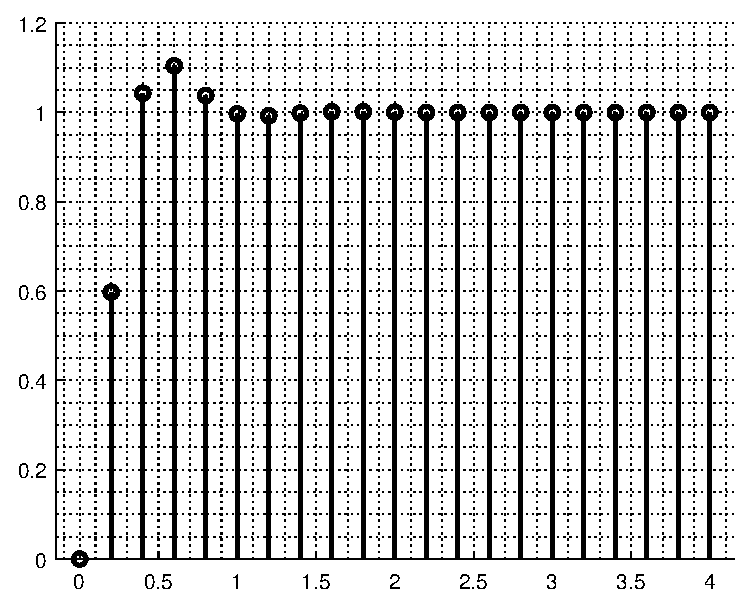
\includegraphics[width=0.75\textwidth]{img/lec10_step1}
    \caption{PID kontrol için kapalı çevrim basamak yanıtı}
    \label{fig:lec10_step1}
\end{figure}

Görüldüğü üzere isterlere oldukça yakın değerler elde edilmiştir. Bunun sebebi, PID kontrolörün fazladan parametreye sahip olması ve bu parametre kullanılarak bir eniyileştirme işleminin mümkün olmasıdır.
\chapter{Z Tanım Bölgesinde Durum Uzayı}

Yay-kütle-damper sisteminin dinamikleri $x(t)$ yer değiştirme olmak üzere
\begin{equation}
    m\ddot{x}(t)+b\dot{x}(t)+kx(t)=u(t)
\end{equation}
ile verilmiştir. Verilen ikinci dereceden diferansiyel denklemi iki adet birinci dereceden diferansiyel denkleme çevirmek mümkündür. Bunun için $x_1(t)\triangleq x(t)$ tanımlanır ve
\begin{equation}
\begin{split}
    \dot{x}_1(t)&=\dot{x}(t)\triangleq x_2(t)\\
    \dot{x}_2(t)&=\ddot{x}(t)
\end{split}
\end{equation}
tanımlanır. Bu durumda,
\begin{equation}
    \begin{split}
        m\ddot{x}(t)+b\dot{x}(t)+kx(t)=u(t)\\
        m\dot{x}_2(t)+bx_2(t)+kx_1(t)=u(t)\\
        m\dot{x}_2(t)=-bx_2(t)-kx_1(t)+u(t)\\
        \dot{x}_2(t)=-\frac{b}{m}x_2(t)-\frac{k}{m}x_1(t)+\frac{1}{m}u(t)
    \end{split}
\end{equation}
elde edilir. Diferansiyel denklem takımı
\begin{equation}
    \begin{split}
        \dot{x}_1(t)&=x_2(t)\\
        \dot{x}_2(t)&=-\frac{b}{m}x_2(t)-\frac{k}{m}x_1(t)+\frac{1}{m}u(t)
    \end{split}
\end{equation}
ve hatta 
\begin{equation}
    \begin{bmatrix}
        \dot{x}_1(t)\\
        \dot{x}_2(t)
    \end{bmatrix}=
    \begin{bmatrix}
        0& 1\\
        -\frac{k}{m}& -\frac{b}{m}
    \end{bmatrix}\begin{bmatrix}
        x_1(t)\\
        x_2(t)
    \end{bmatrix}+\begin{bmatrix}
        0\\
        \frac{1}{m}
    \end{bmatrix}u(t)
\end{equation}
elde edilir. Sistem için parametreler $m=1$, $b=0.5$ ve $k=1$ olmak üzere durum uzayı modeli
\begin{equation}
\begin{split}
    \begin{bmatrix}
        \dot{x}_1(t)\\
        \dot{x}_2(t)
    \end{bmatrix}&=
    \begin{bmatrix}
        0& 1\\
        -1& -0.5
    \end{bmatrix}\begin{bmatrix}
        x_1(t)\\
        x_2(t)
    \end{bmatrix}+\begin{bmatrix}
        0\\
        1
    \end{bmatrix}u(t)\\
    y(t)&=\begin{bmatrix}
        1&0 
    \end{bmatrix}\begin{bmatrix}
        x_1(t)\\
        x_2(t)
    \end{bmatrix}
\end{split}
\end{equation}
olarak elde edilir. \verb|Simulink| modeli Şekil~\ref{fig:model1} ile verilmiştir.
\begin{figure}[!htb]
    \centering
    \includegraphics[width=\textwidth]{img/model1}
    \caption{Yay-kütle-damper sistemine ait durum uzay modeli}
    \label{fig:model1}
\end{figure}

Ayrık durum uzayı ZOH yöntemi ile türevin yorumuna dayanmaktadır ve 
\begin{equation}
    \frac{dx}{dt}=\frac{\Delta x}{\Delta t}=\frac{x(kT)-x((k-1)T)}{T}
\end{equation}
ile durum uzayı
\begin{equation}
    \begin{split}
        \frac{1}{T}\begin{bmatrix}
            x_1(kT)-x_1((k-1)T)\\
            x_2(kT)-x_2((k-1)T)
        \end{bmatrix}&=
        \begin{bmatrix}
            0& 1\\
            -1& -0.5
        \end{bmatrix}\begin{bmatrix}
            x_1((k-1)T)\\
            x_2((k-1)T)
        \end{bmatrix}+\begin{bmatrix}
            0\\
            1
        \end{bmatrix}u((k-1)T)\\
        y((k-1)T)&=\begin{bmatrix}
            1&0 
        \end{bmatrix}\begin{bmatrix}
            x_1((k-1)T)\\
            x_2((k-1)T)
        \end{bmatrix}
    \end{split}
\end{equation}
olarak elde edilmektedir. Matematiksel işlemler sonucu
\begin{equation}
    \begin{split}
        \begin{bmatrix}
            x_1(kT)\\
            x_2(kT)
        \end{bmatrix}&=
        \begin{bmatrix}
            1&0\\
            0&1
        \end{bmatrix}
        \begin{bmatrix}
            x_1((k-1)T)\\
            x_2((k-1)T)
        \end{bmatrix}+
        T\begin{bmatrix}
            0& 1\\
            -1& -0.5
        \end{bmatrix}\begin{bmatrix}
            x_1((k-1)T)\\
            x_2((k-1)T)
        \end{bmatrix}+\begin{bmatrix}
            0\\
            T
        \end{bmatrix}u((k-1)T)\\
        y((k-1)T)&=\begin{bmatrix}
            1&0 
        \end{bmatrix}\begin{bmatrix}
            x_1((k-1)T)\\
            x_2((k-1)T)
        \end{bmatrix}
    \end{split}
    \end{equation}
    ve sonuç olarak
        \begin{equation}
            \begin{split}
        \begin{bmatrix}
            x_1(kT)\\
            x_2(kT)
        \end{bmatrix}&=
        \begin{bmatrix}
            1& T\\
            -T& 1-0.5T
        \end{bmatrix}\begin{bmatrix}
            x_1((k-1)T)\\
            x_2((k-1)T)
        \end{bmatrix}+\begin{bmatrix}
            0\\
            T
        \end{bmatrix}u((k-1)T)\\
        y((k-1)T)&=\begin{bmatrix}
            1&0 
        \end{bmatrix}\begin{bmatrix}
            x_1((k-1)T)\\
            x_2((k-1)T)
        \end{bmatrix}\\
    \end{split}
\end{equation}
elde edilir. Örnekleme zamanı $T=0.1$ olmak üzere durum uzayı modeli
\begin{equation}
    \begin{split}
\begin{bmatrix}
    x_1[k]\\
    x_2[k]
\end{bmatrix}&=
\begin{bmatrix}
    1& 0.1\\
    -0.1& 0.95
\end{bmatrix}\begin{bmatrix}
    x_1[k-1]\\
    x_2[k-1]
\end{bmatrix}+\begin{bmatrix}
    0\\
    0.1
\end{bmatrix}u[k-1]\\
y[k-1]&=\begin{bmatrix}
    1&0 
\end{bmatrix}\begin{bmatrix}
    x_1[k-1]\\
    x_2[k-1]
\end{bmatrix}\\
\end{split}
\end{equation}
şeklindedir. Durum uzayı modeli denklemleri
\begin{equation}
    \begin{split}
    x_1[k]&=x_1[k-1]+0.1x_2[k-1]\\
    x_2[k]&=-0.1x_1[k-1]+0.95x_2[k-1]+0.1u[k-1]\\
    y[k-1]&=x_1[k-1]
\end{split}
\end{equation}
şeklindedir. Girişine $sin(4t)$ uygulandığında elde edilen yanıt Şekil~\ref{fig:lec11_plot1} ile verilmiştir.
\begin{figure}[!htb]
    \centering
    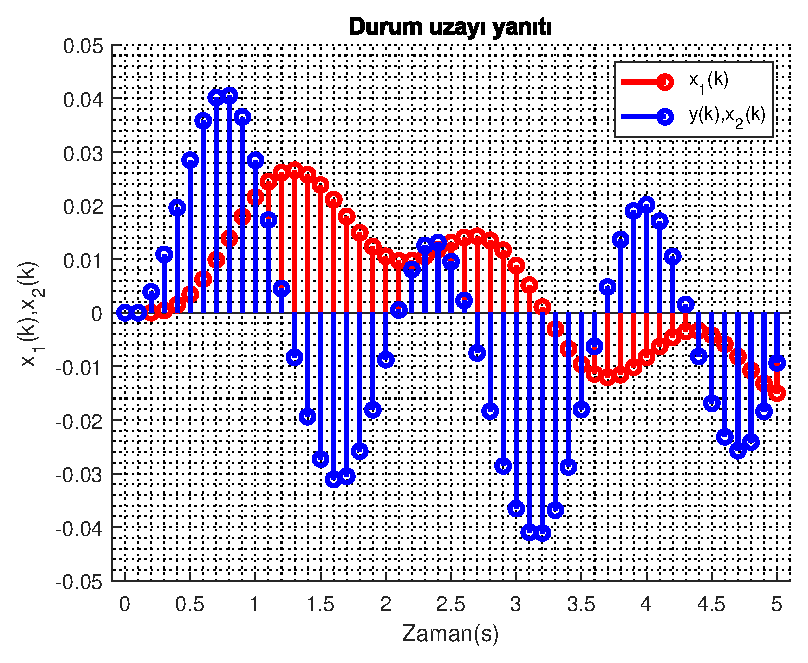
\includegraphics[width=0.75\textwidth]{img/lec11_plot1}
    \caption{Yay-kütle-damper sistemine ait durum uzay modeli yanıtı}
    \label{fig:lec11_plot1}
\end{figure}

\verb|Simulink| modeli Şekil~\ref{fig:model2} ile verilmiştir.
\begin{figure}[!htb]
    \centering
    \includegraphics[width=\textwidth]{img/model2}
    \caption{Yay-kütle-damper sistemine ait ayrık durum uzay modeli}
    \label{fig:model2}
\end{figure}

\chapter{Z Tanım Bölgesinde Durum Geri Besleme Kontrolörü}
Durum uzay modeli
\begin{equation}
    x(k)=A x(k-1)+Bu(k-1),\quad y(k-1)=C x(k-1)
\end{equation}
olmak üzere 
\begin{equation}
    u(k-1)=K x(k-1)
\end{equation}
kontrolörüne \textbf{Durum Geri Besleme} kontrolörü adı verilmektedir. Dikkat edilirse bu kontrol kuralı
\begin{equation}
\begin{split}
    u(k-1)&=K x(k-1)\\
    u(k-1)&=\begin{bmatrix}k_1& k_2& \cdots& k_n\end{bmatrix} \begin{bmatrix}x_1(k-1)\\x_2(k-1)\\\vdots\\x_n(k-1)\end{bmatrix}\\
    u(k-1)&=k_1x_1(k-1)+k_2x_2(k-1)+\cdots+k_nx_n(k-1)
\end{split}
\end{equation}
olarak yazılabilir. Bu kontrolör ile kapalı çevrim durum uzay modeli
\begin{equation}
    \begin{split}
        x(k)&=A x(k-1)+Bu(k-1),\quad y(k-1)=C x(k-1)\\
        x(k)&=A x(k-1)+BKx(k-1),\quad y(k-1)=C x(k-1)\\
        x(k)&=(A+BK) x(k-1),\quad y(k-1)=C x(k-1)
    \end{split}
\end{equation}
olarak elde edilir. Kapalı çevrim modelin z tanım bölgesi ifadesi
\begin{equation}
    \begin{split}
        x(k)&=(A+BK) x(k-1)+B r(k-1),\quad y(k-1)=C x(k-1)\\
        z^1 x(k-1)&=(A+BK) x(k-1)+B r(k-1),\quad y(k-1)=C x(k-1)\\
        (zI-(A+BK)) x(k-1)&=B r(k-1),\quad y(k-1)=C x(k-1)\\
        x(k-1)&=(zI-(A+BK))^{-1} B r(k-1),\quad y(k-1)=C x(k-1)\\
        y(k-1)&=C(zI-(A+BK))^{-1}B r(k-1)\\
        \frac{y(k-1)}{r(k-1)}&=C(zI-(A+BK))^{-1}B
    \end{split}
\end{equation}
şeklindedir ve karakteristik polinom
\begin{equation}
    \begin{split}
        p_c(z)=det(zI-(A+BK))
    \end{split}
\end{equation}
ile hesaplanır.


\chapter{Z Tanım Bölgesinde Luenberger Gözleyicisi}


\end{document}
